
A comparison of force response in the form of normalized lift and drag forces is shown in Figures \ref{fig:lift_zonal_adapt_Re200k} and \ref{fig:drag_zonal_adapt_Re200k} respectively. 
At $\psi=90^\circ$, maximum lift is achieved for all meshes.
This maximum lift is smaller for M0\_nz50 as compared to other meshes. 
Lift for Mza1 and Mza2 meshes compare well with each other.
Normalized drag compares well with each other for all meshes considered.

\begin{figure}[H]
	\centering
	
	\begin{subfigure}[b]{0.7\textwidth}
		\centering
		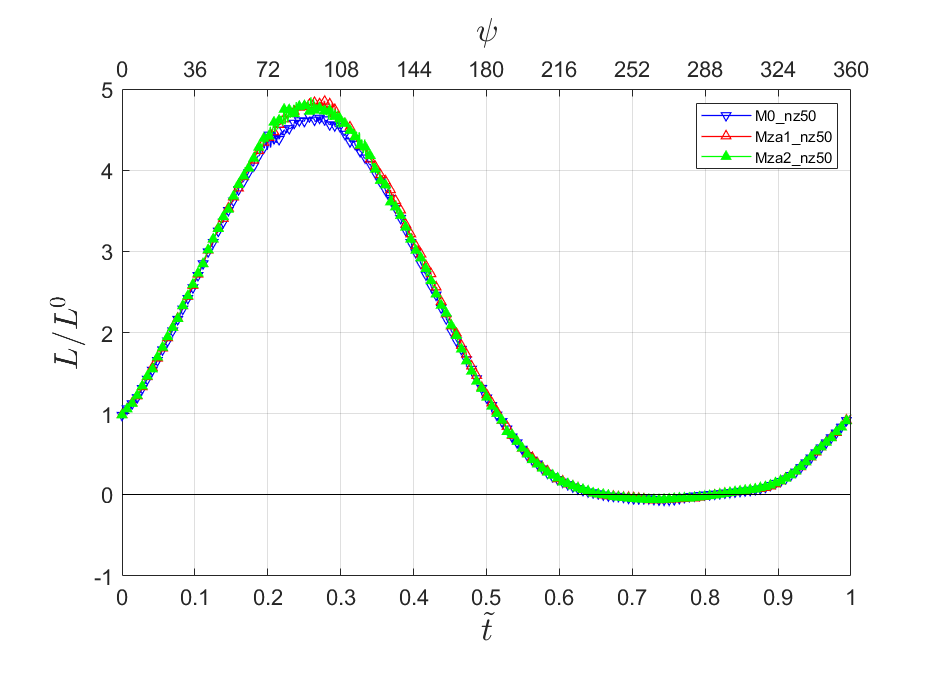
\includegraphics[width=1\textwidth]{figures/zonal_adapt_results/force_response_Re200k/Lift_inst.png}
		\caption{Normalized lift}
		\label{fig:lift_zonal_adapt_Re200k}
	\end{subfigure}
	\begin{subfigure}[b]{0.7\textwidth}
		\centering
		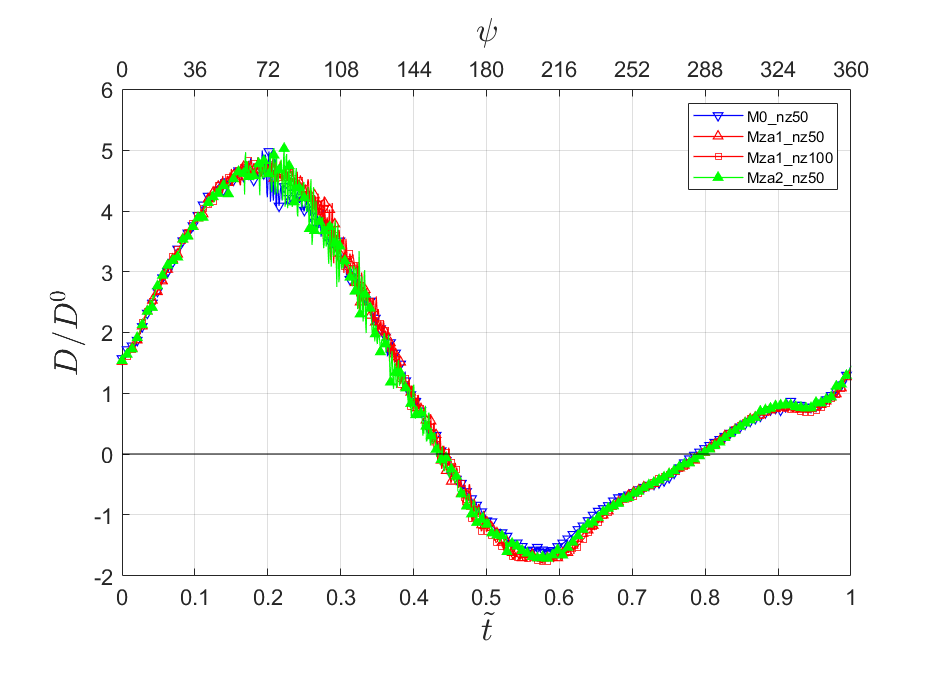
\includegraphics[width=1\textwidth]{figures/zonal_adapt_results/force_response_Re200k/Drag_inst.png}
		\caption{Normalized drag}
		\label{fig:drag_zonal_adapt_Re200k}
	\end{subfigure}
	
	\label{fig:force_response_zonal_adapt_Re200k}
	\caption{Normalized forces for different meshes}
\end{figure}